\chapter{Experimental Work}
\label{ch:experimental_work}
This chapter describes the experimental work done as part of the project. Since it is a rather incremental process, the goal, procedure and relevant results are described individually in each section.

\section{Implementation of a Runtime Support System for State Machines in Lua}
\label{sec:impl_runtime_support}
The first step towards working with state machine -based applications, is building a runtime system for a collection of generalized state machines. For the experimental purposes of this project, a runtime system with only the most basic functionality is needed. The components required for this are:

\begin{itemize}
	\item An \guillemotleft event\guillemotright  data structure for handling messages to and between state machines
	\item A \guillemotleft timer\guillemotright  object for keeping track of timed events
	\item A prototype/\gls{api} for state machines
	\item A \guillemotleft scheduler\guillemotright  to keep track of active state machines, events and timers, and assigning events and timers to their respective state machines at the appropriate time.
\end{itemize}

It turns out to be quite simple to implement this system in Lua. The source code is included in Appx.~\ref{code:rts}, and each component is explained in the sections below.

\subsection{Event Data Structure}
\label{sec:impl_event}
Even though Lua is not natively object-oriented, an event object is still easily implemented by use of the \emph{\_\_index} metamethod~\cite[13.4.1]{book:programming_in_lua_first}. We simply create a prototype for the event object with the desired fields (ID of state machine, event type and additional data) and methods (constructor, setters and getters). Inheritance is then enabled by creating an empty table/object, and setting its \emph{\_\_index} to reference the parent object's fields. Lua doesn't support encapsulation by conventional means~\cite[16.4]{book:programming_in_lua_first}, but rather by creating \emph{closures}. Encapsulated fields may then only be accessed by functions declared in the same local scope, as seen in the constructor method for event (\emph{Event:new}, Code snip.~\ref{code:event}). This is useful also in a state machine context to avoid inadvertent or even malicious tampering with event data or state of state machines. Combined, these approaches make the event data structure simple, safe and easy to use.

\subsection{Timer Object}
\label{sec:impl_timer}
The timer object (Code snip.~\ref{code:timer}) is created similarly to the event object described in Sect.~\ref{sec:impl_event} with respect to inheritance and encapsulation. Additionally, we need some way to keep track of time. As discussed in Sect.~\ref{sec:lua_and_state_machines}, Lua does not natively offer preemptive multitasking, so running an active timer on a separate thread is pretty much out of the question. However, for a simple runtime system, we may delegate the responsibility of measuring time to the scheduler component, and simply create a \guillemotleft timestamp\guillemotright  for the desired activation time. This may decrease the timing accuracy of activation, but on the other hand also decreases overhead and complexity of the runtime system. In many cases it is not necessary or even desirable to preempt a running transition, but sufficient to wait until the transition has finished before scheduling the event following the timeout. This is however something that should be addressed when designing a more complete runtime system, and something that may prove challenging, as discussed in Sect.~\ref{sec:lua_and_state_machines}.

The granularity of the timestamp is another issue that must be addressed, and is also discussed in Sect.~\ref{sec:lua_and_state_machines}. As a starting point, I chose to use \emph{os.time()}, even though it only offers \emph{second}-granularity. This is OK for the preliminary examples, and further addressed in Sect.~\ref{sec:running_on_micro}.

\subsection{State Machine Prototype/API}
\label{sec:impl_stm}
The third component we need is a prototype for implementation of a given state machine. This prototype serves as a kind of API, defining some common values and methods for all state machines. The state machine prototype (Code snip.~\ref{code:stm}), inspired by an exercise given in the course TTM4160 at NTNU, contains some predefined values to be returned to the scheduler after a transition, encapsulated data fields for state and ID, as well as a \guillemotleft fire\guillemotright  function meant to be overridden in an implementation. When overridden, this function should implement all possible transitions for the state machine inside an eternal \emph{while}-loop such that only one transition is executed each pass.

Additionally, the required presence of a \guillemotleft run\guillemotright  field holding a coroutine is indicated. The coroutine scheme is probably what makes the Lua implementation most unique. The coroutine references the \guillemotleft fire\guillemotright  function, causing this function to be \emph{resumed} when the coroutine is resumed. This coroutine scheme fits perfectly into our runtime system as a way of structuring the program. Each state machine has its own coroutine with a separate thread, maintaining its state as well as other data, while the scheduler (see Sect. \ref{sec:impl_sched}) runs the main thread, handing execution control over to state machines according to events and timeouts. As a result of this, a state machine transition is never interrupted by a scheduler, meaning we have to trust all state machines to eventually hand execution control back to the scheduler. On the other hand, we don't have to worry about making state machines or transitions \guillemotleft thread safe\guillemotright .

\subsection{Scheduler}
\label{sec:impl_sched}
The scheduler (Code snip.~\ref{code:scheduler}) is the last component we need for our runtime system, and this is where the flexible properties of Lua tables really come into play. The scheduler needs to provide a set of functions enabling the following:

\begin{itemize}
	\item Adding and removing state machines
	\item Adding and keeping track of new events
	\item Adding, removing (stopping) and keeping track of timers
	\item Scheduling of events and timers (timeouts) to their respective state machines in an appropriate order
\end{itemize}

Adding and removing state machines is enabled by keeping a table with references to active state machine objects, indexed by their ID. Similar schemes are implemented for events and timers. Lua tables natively allow indexing by arbitrary values, as well as inserting at the end or removing from the front, effectively emulating the semantics of a hashmap or a queue without the need for any extra tweaking or import of libraries. The list of timers is kept sorted to make checking for timeouts quicker, but at the cost of extra work on insertion (with busy waiting, checking timers is generally done a lot more often than adding new timers).

Finally, we have a continuously running \guillemotleft run\guillemotright  function that handles the actual scheduling. The scheduling scheme is kept simple: timeouts have priority over events. For each pass, the function first checks if any timers have expired, and if not, moves on to check if there are any events waiting. If a timeout or event is found, execution control is handed to the state machine it belongs to with a \emph{coroutine.resume} call. The scheduler thread then waits until the following transition is completed, and execution control is returned from the state machine through the \emph{coroutine.yield} call, before doing another pass.

\subsection{Missing Features and Possible Issues}
While the most basic functionality is easy to implement, the runtime system outlined in the previous sections far from complete. It is probably sufficient for very basic state machine applications that don't have, for example, strict timing requirements or external event sources. These issues should be considered when designing a more complete system.

\paragraph{Multitasking} The main issue to consider here is probably multitasking. For a simple scheme where only the internal state machines are generating events, non-preemptive multitasking is a great solution. However, in many cases sources of events will be external to the system like in the case of an Ethernet socket. With only one thread executing at a time, receiving external events asynchronously is difficult. Most likely we need another process running in parallel, listening for events and adding them to the queue as they arrive, which in most cases means preemptive multitasking, however shared memory/pipes may also be an option. Additionally, an ill-defined state machine may get stuck in a transition, never returning control to the scheduler. In this case, it could have been wise to have a \guillemotleft watchdog\guillemotright timer running in parallel, ready to hand control back to the scheduler if the transition takes too long. Standard Lua does not offer any way of doing this though, so our options are to use external libraries or write our own multitasking module. Some Lua libraries implementing preemptive multitasking exist, but I have left these out for now, as they rely on threads in the underlying operating system, which will not be available when we move on to the microcontroller in Sect.~\ref{sec:running_on_micro}.

\paragraph{Timing Accuracy} Another point we need to consider, is timeout accuracy. Since timers are not allowed to preempt, execution may be delayed for an unknown amount of time. Again, this is probably ok if you don't require very strict timing accuracy, but this may not always be the case. Unfortunately, better guarantees for timing accuracy is hard to achieve without preemptive multitasking.

\paragraph{Saving Events}

\paragraph{Busy Waiting}

\section{Implementation of State Machines in Lua}
\label{sec:impl_state_machines}
When we have a working runtime system, the next step is to create state machines implementing the application we want to create. The following sections provide some examples of simple state machine applications, based on the prototype described in Sect.~\ref{sec:impl_stm}.

\subsection{The Traffic Light Controller State Machine}
\label{sec:impl_traffic_light}
Like the state machine prototype, the Traffic Light Controller is inspired by an exercise given in the TTM4160 course. In this application, we simulate a controller for a pedestrian traffic light. When a pedestrian pushes the button, the light for cars is set to yellow, and a timer is started. Following the resulting timeout, lights are set to new colors and new timers are started accordingly, until the whole sequence is complete, and the controller waits for a new button press. Its \gls{uml} specification is shown in Fig.~\ref{fig:traffic_light_uml}, and the resulting Lua code in Code snip.~\ref{code:traffic_light}.

The Lua code is fairly straightforward: we load required modules and define some constants specific to this state machine, like states, timer delays, and event types. The next step is to create a simple constructor, assigning a given ID to the new Traffic Light Controller instance, setting the initial state, and keeping a reference to the scheduler. The final part is the \emph{fire} function looping over all the possible transitions. This is implemented in an action-oriented way, making the code clearly structured and very readable. Every transition fork ends with a call to \emph{coroutine.yield}, handling execution control back to the scheduler. It is really important to end every possible fork with a yield as done with the numerous \emph{else} statements, or we risk the state machine getting stuck in the loop in case of an unexpected event.

Testing the application is equally straightforward: we create a \guillemotleft main\guillemotright  program (Code snip.~\ref{code:main}) with an instance of the scheduler and the Traffic Light controller, and register the state machine with the scheduler. We also create a \guillemotleft fake\guillemotright  button press event, and add it to the scheduler's event queue. Finally, we start the runtime system by calling the scheduler's \emph{run} function, and observe the following behavior.

A test run of this application provided the output displayed in Fig.~\ref{fig:traffic_light_output}, with the appropriate timer delays between each line. This is in line with what we would expect from the \gls{uml} specification in Fig.~\ref{fig:traffic_light_uml}.

\begin{figure}[H]
	\centering
	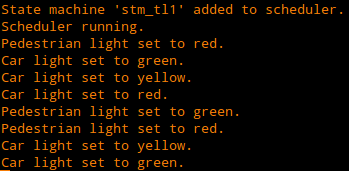
\includegraphics[scale=0.70]{traffic_light_output}
	\caption[Output of Traffic Light Controller test run]{Console output resulting from the test run of the Traffic Light Controller state machine application.}
	\label{fig:traffic_light_output}
\end{figure}

\subsection{Two Communicating Applications}


\subsection{Comparison to Generated State Machines}


\section{Running the State Machine -based Application on a Microcontroller}
\label{sec:running_on_micro}

\subsection{The LM3S9D92 Microcontroller}

\subsection{Running eLua on the Evaluation Kit Board}

\subsection{Running the Simple Application}

\section{Measurements of RTS performance Overhead}
\label{sec:overhead_measure}

\begin{listing}[H]
\begin{luacode}
local task_size = 10
local task_repeats = 1

local function busy_work()
	for i=1,task_size do
		q = i*i
	end
end

local start_time = tmr.read(tmr.SYS_TIMER)

for j=1,task_repeats do
	busy_work()
end

local delta = tmr.read(tmr.SYS_TIMER) - start_time
print("Delta: "..tostring(delta))
\end{luacode}
	\caption{Lua code used for overhead testing}
	\label{code:overhead}
\end{listing}

\section{Measurements of Application Performance}
\label{sec:performance_measure}

